\taskpic{ На поверхность воды бросают три кусочка нитки, связанных
  так, как показано на рисунке. Длина двух одинаковых кусочков $l_1 +
  l_3 = 3$ см, а $l_2=1$ см. В точках $A$ и $B$ капают
  поверхностно--активное вещество, которое снижает коэффициент
  поверхностного натяжения воды в $n=2{,}5$ раза. Каким будет
  натяжение каждого из кусков? }
{
  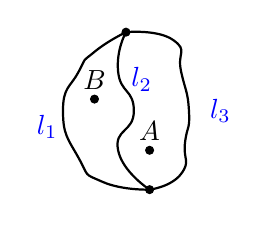
\begin{tikzpicture}
    \draw[thick] plot [smooth,tension=1] coordinates {(2,2) (1.9,1.5)
      (2.1,1) (1.9,0.5) (2.3,0)} node at (2,0) {};
    \draw[thick] plot [smooth,tension=1] coordinates {(2,2)
      (1.6,1.75) (1.4,1.5) (1.2,1) (1.4,0.4) (1.7,0.1) (2.3,0)} node
    at (2,0) {};    
    \draw[thick] plot [smooth,tension=1] coordinates {(2,2)
      (2.6,1.9) (2.7,1.5) (2.8,1) (2.75,0.6) (2.7,0.2) (2.3,0)} node at
    (2,0) {};
    \draw[fill=black] (2,2) circle (0.05cm) (2.3,0) circle (0.05cm);
    \draw[blue] (3.2,1) node {$l_3$};
    \draw[blue] (1,0.8) node {$l_1$};
    \draw[blue] (2.2,1.4) node {$l_2$};
    \draw[fill=black] (1.6,1.15) circle (0.05cm) node[above] {$B$};
    \draw[fill=black] (2.3,0.5) circle (0.05cm) node[above] {$A$};
  \end{tikzpicture}
}
% Раз задача, два задача, 2.38